\section{CFR: a little regret-matcher at every decision point}\label{sec:cfr}

\mkey{counterfactual regret}Regret matching handles one simultaneous decision. Poker is a \emph{tree} of sequential decisions under hidden information, and the naive fix --- treat every complete game plan as one giant ``action'' and regret-match over plans --- explodes combinatorially. The 2007 breakthrough of Zinkevich, Johanson, Bowling, and Piccione~\cite{zinkevich2007} is \keyterm{counterfactual regret minimization}\mdef{CFR}{run an independent regret-matcher at every infoset; their local regrets provably bound global regret}: put an \emph{independent} little regret ledger at every information set, define each one's regret the right way, and prove the sum of the local regrets upper-bounds the global regret of the whole strategy. Minimize locally, win globally --- then the folk theorem from Section~\ref{sec:rm} converts the vanishing regret into a converging \emph{average} strategy.

The one subtlety is what ``the right way'' means, and it is where the name comes from.

\begin{intuition}{counterfactual value: score the spot as if you had steered to it}
An infoset deep in the tree is only reached some of the time, and partly because of \emph{your own} earlier choices. If local regrets were weighted by how often \emph{you} actually go there, a spot you currently avoid would accumulate no regret and never be reconsidered --- learning would freeze. So CFR scores each infoset \emph{counterfactually}: weight its value by the probability that \emph{the opponent and the deck} let you arrive (their reach), while pretending you steered there with probability one. Your own choices never gate their own reconsideration; the opponent's play and the cards set the stakes. That reach-weighting detail is the entire trick --- and getting it backwards is the classic silent implementation bug (Section~\ref{sec:engineering}).
\end{intuition}

In symbols, for infoset $I$ with strategy $\sigma_t$ at iteration $t$, action $a$'s instantaneous regret is
$$ r_t(I,a) \;=\; \pi^{\sigma_t}_{-i}(I)\,\bigl[\,v(I,a) - \textstyle\sum_{a'} \sigma_t(I,a')\,v(I,a')\,\bigr], $$
where $\pi^{\sigma_t}_{-i}(I)$ is the opponent-and-chance reach probability and $v(I,a)$ the expected payoff after taking $a$ at $I$. Each ledger accumulates $R_T(I,a)=\sum_t r_t(I,a)$; regret matching over $R_T^+$ gives the next strategy; and the guarantee is exploitability of the \emph{average} strategy shrinking as $O(1/\sqrt{T})$.

\begin{lstlisting}
def cfr(state, reach_me, reach_opp):         # one traversal, my update
    if state.terminal(): return state.payoff()
    I = infoset(state)                        # my cards + public history
    sigma = regret_match(ledger[I])
    v = {a: cfr(state.play(a), ...) for a in I.actions}   # recurse
    ev = sum(sigma[a] * v[a] for a in I.actions)
    if I.player == me:
        for a in I.actions:                   # counterfactual weighting
            ledger[I][a]     += reach_opp * (v[a] - ev)
        avg_ledger[I][sigma] += reach_me      # average strategy, own reach
    return ev
\end{lstlisting}

\mkey{kuhn poker}The standard first proving ground is \keyterm{Kuhn poker}\mdef{Kuhn poker}{3-card deck (J,Q,K), one card each, one bet of 1; the smallest real poker game}: twelve infosets, yet genuine hidden information, value betting, and an equilibrium that \emph{must} bluff (the jack bluffs one-third as often as the king value-bets). Its equilibrium is known in closed form, so an implementation can be checked to the digit. Figure~\ref{fig:kuhn} shows CFR solving it live for this paper, and the plot restates every claim of the last two sections with real data: the average strategy's exploitability marches down the $1/\sqrt{T}$ guide toward zero; the \emph{current} strategy of vanilla CFR stays stuck around $0.2$ chips/hand forever, cycling exactly as the theory predicts.\mnote{The simulation behind Fig.~\ref{fig:kuhn} reproduces Kuhn's game value $-1/18\approx-0.0556$ for the first player to 4 decimal places --- the kind of closed-form check Section~\ref{sec:engineering} argues every implementation needs.}

\begin{figure}[t]
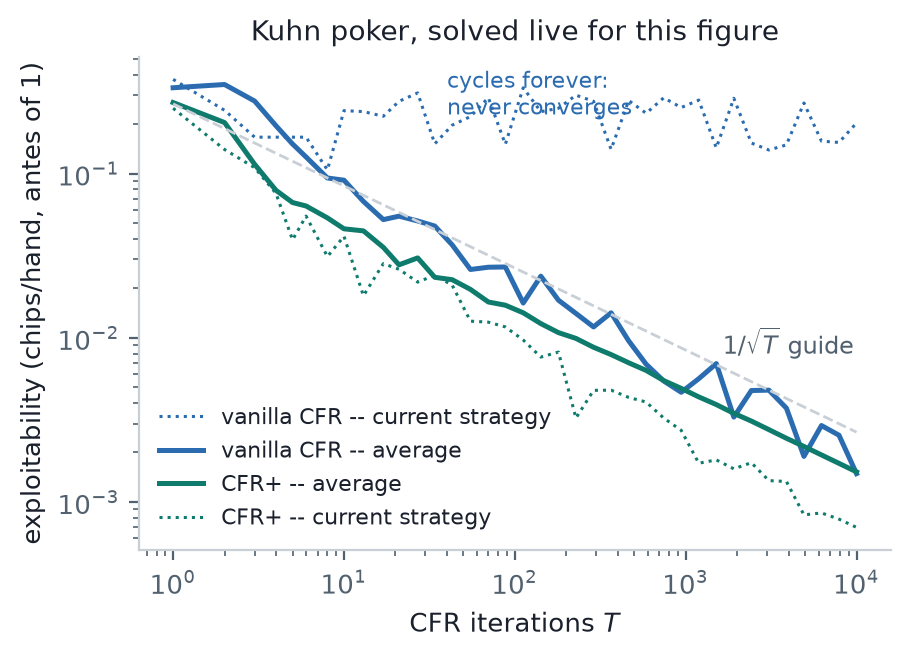
\includegraphics[width=\linewidth]{figures/kuhn_cfr.png}
\caption{Real CFR runs on Kuhn poker (computed for this paper): average-strategy exploitability converges; current strategy either cycles (vanilla) or, under CFR+, converges on its own.}
\label{fig:kuhn}
\end{figure}

The figure also previews the next section: the teal curves are \keyterm{CFR+}, a three-tweak variant whose \emph{current} strategy ends up less exploitable than either average --- the empirical surprise that made million-fold-larger games solvable.

Two closing notes calibrate expectations. First, cost: vanilla CFR walks the \emph{entire} tree every iteration --- fine for Kuhn's 58 nodes, unthinkable for Drawmaha's $10^{12}$ deals; Sections~\ref{sec:speedups}--\ref{sec:mccfr} are the escape routes. Second, memory: CFR stores two numbers per infoset-action (regret sum, strategy sum). That linear-in-infosets footprint is precisely what made $10^{12}$-state abstractions of limit hold'em solvable in 2007 where LP solvers managed $10^{8}$ --- and precisely what runs out at Drawmaha scale, forcing Section~\ref{sec:deepcfr}.
